
\documentclass[12pt,halfline,a4paper,]{ouparticle}

% Packages I think are necessary for basic Rmarkdown functionality
\usepackage{hyperref}
\usepackage{graphicx}
\usepackage{listings}
\usepackage{xcolor}
\usepackage{fancyvrb}
\usepackage{framed}

% Link coloring
\hypersetup{breaklinks=true,
            bookmarks=true,
            pdfauthor={},
            pdftitle={STA2005S - Experimental Design Assignment}
            }


%% To allow better options for figure placement
%\usepackage{float}

% Packages that are supposedly required by OUP sty file
\usepackage{amssymb, amsmath, geometry, amsfonts, verbatim, endnotes, setspace}

% use upquote if available, for straight quotes in verbatim environments
\IfFileExists{upquote.sty}{\usepackage{upquote}}{}

% Macros for dealing with affiliations, footnotes, etc.
\makeatletter
\def\Newlabel#1#2#3{\expandafter\gdef\csname #1@#2\endcsname{#3}}

\def\Ref#1#2{\@ifundefined{#1@#2}{???}{\csname #1@#2\endcsname}}

\newcommand*\samethanks[1][\value{footnote}]{\footnotemark[#1]}

\newcommand*\ifcounter[1]{%
  \ifcsname c@#1\endcsname
    \expandafter\@firstoftwo
  \else
    \expandafter\@secondoftwo
  \fi
}

\newcommand*\thanksbycode[1]{%
  \ifcounter{FNCT@#1}
    {\samethanks[\value{FNCT@#1}]}
    {\thanks{\Ref{FN}{#1}}\newcounter{FNCT@#1}\setcounter{FNCT@#1}{\value{footnote}}}
}

% Create labels for Addresses if the are given in Elsevier format

% Create labels for Footnotes if the are given in Elsevier format

% Part for setting citation format package: natbib

% Part for setting citation format package: biblatex


% tightlist command for lists without linebreak
\providecommand{\tightlist}{%
  \setlength{\itemsep}{0pt}\setlength{\parskip}{0pt}}

% From pandoc table feature
\usepackage{longtable,booktabs,array}
\usepackage{calc} % for calculating minipage widths
% Correct order of tables after \paragraph or \subparagraph
\usepackage{etoolbox}
\makeatletter
\patchcmd\longtable{\par}{\if@noskipsec\mbox{}\fi\par}{}{}
\makeatother
% Allow footnotes in longtable head/foot
\IfFileExists{footnotehyper.sty}{\usepackage{footnotehyper}}{\usepackage{footnote}}
\makesavenoteenv{longtable}


\usepackage{booktabs}
\usepackage{longtable}
\usepackage{array}
\usepackage{multirow}
\usepackage{wrapfig}
\usepackage{float}
\usepackage{colortbl}
\usepackage{pdflscape}
\usepackage{tabu}
\usepackage{threeparttable}
\usepackage{threeparttablex}
\usepackage[normalem]{ulem}
\usepackage{makecell}
\usepackage{xcolor}

\begin{document}

\title{STA2005S - Experimental Design Assignment}

\author{%
%
% Code for old style authors field
%
% Add \and if both authors and author
%
%
% Code for new (elsevier) style author field
\name{Jing Yeh}
\address{\Ref{ADR}{University of Cape Town}}
%
\email{\href{mailto:yhxjin001@myuct.ac.za}{yhxjin001@myuct.ac.za}}%
%
%
%
\and
\name{Saurav Sathnarayan}
\address{\Ref{ADR}{University of Cape Town}}
%
\email{\href{mailto:yhxjin001@myuct.ac.za}{yhxjin001@myuct.ac.za}}%
%
%
%
%
}

\abstract{Test}

\date{2024-09-13}

\keywords{key; dictionary; word}

\maketitle



\newpage

\section{Introduction}\label{introduction}

Computation has been playing a major role in human history ever since
people began living in cities. The need to calculate taxes motivated the
invention of various computing devices that aided such computations,
such as the Sumerian abacus, invented in Babylon at around
2500BC{[}7{]}. In the 21st century, the capability our digital computing
devices have vastly surpassed the capacity of those proto-computers, but
so has our need for computational power. Everything in our daily life
requires some form of computers: from our phones, cars, to even our
refrigerators (side note: initially, Java was actually invented for
refrigerators).

However, with large computation capability comes the complexity in the
design of these device: to speak plainly, they are damn difficult to
use. Computer scientists have therefore invented numerous
\emph{programming languages} that allow us to harness the power of these
devices more easily.

Eventually, programming languages have become the primary medium for
instructing computers to perform our increasingly complex tasks.
Understanding which programming languages offer superior execution speed
is therefore crucial for developers, especially in domains requiring
real-time processing, large-scale data analysis, and other
resource-intensive computations. The goal of this experiment is to
identify such languages that deliver the fastest execution time.

\textbf{when calculating a value of \(\pi\) with respect to Leibiniz
formula. \[\sum_{n=0}^{\infty} (-1)^n/(2n+1)\]}

This problem will focus on evaluating a selection of popular programming
languages, including but not limited to C++, C, R, Python, Java, and
Ruby. The evaluation will consider how quickly a value of pi can be
calculated by applying leibiniz formula up to 100000000 terms.\\

\subsection{Compiled vs Interpreted
Languages}\label{compiled-vs-interpreted-languages}

\paragraph{Compiled Language:}\label{compiled-language}

\hfill\break
In a compiled language, the source code is translated into machine code
by a compiler before execution. This machine code, often called an
executable, can be run directly by the computer's hardware.\\
Compiled programs typically run faster since they are already in machine
language, which the computer's processor can execute directly.\\
Examples: C, C++, Rust, and Go are examples of compiled languages.

\paragraph{Interpreted Language:}\label{interpreted-language}

\hfill\break
In an interpreted language, the source code is executed line-by-line by
an interpreter at runtime. The interpreter reads the code, translates it
into machine code, and executes it on the fly.\\
Interpreted programs generally run slower than compiled ones because the
translation happens during execution.\\
Examples: Python, JavaScript, Ruby, and PHP are examples of interpreted
languages.

\paragraph{Key Differences:}\label{key-differences}

Compiled languages require a compilation step that produces an
executable, while interpreted languages are executed directly by an
interpreter.\\
Compiled languages tend to have better performance due to the
pre-compiled nature of the code, whereas interpreted languages are more
flexible but slower due to the runtime translation.\\
Some languages, like Java, use a combination of both techniques, where
the code is first compiled into an intermediate form (bytecode) and then
interpreted just-in-time (JIT) at runtime.\\

\subsection{A Priori Analysis}\label{a-priori-analysis}

Since existing literature on the execution times of programming
languages when applying Leibniz's formula is limited, we performed an a
priori test to gauge the execution time for the programming languages we
planned on experimenting with. We performed 500 approximations of \(pi\)
,using the algorithm described in the Method section, for each
programming language. We obtained the following jittered graph.\\
\strut \\

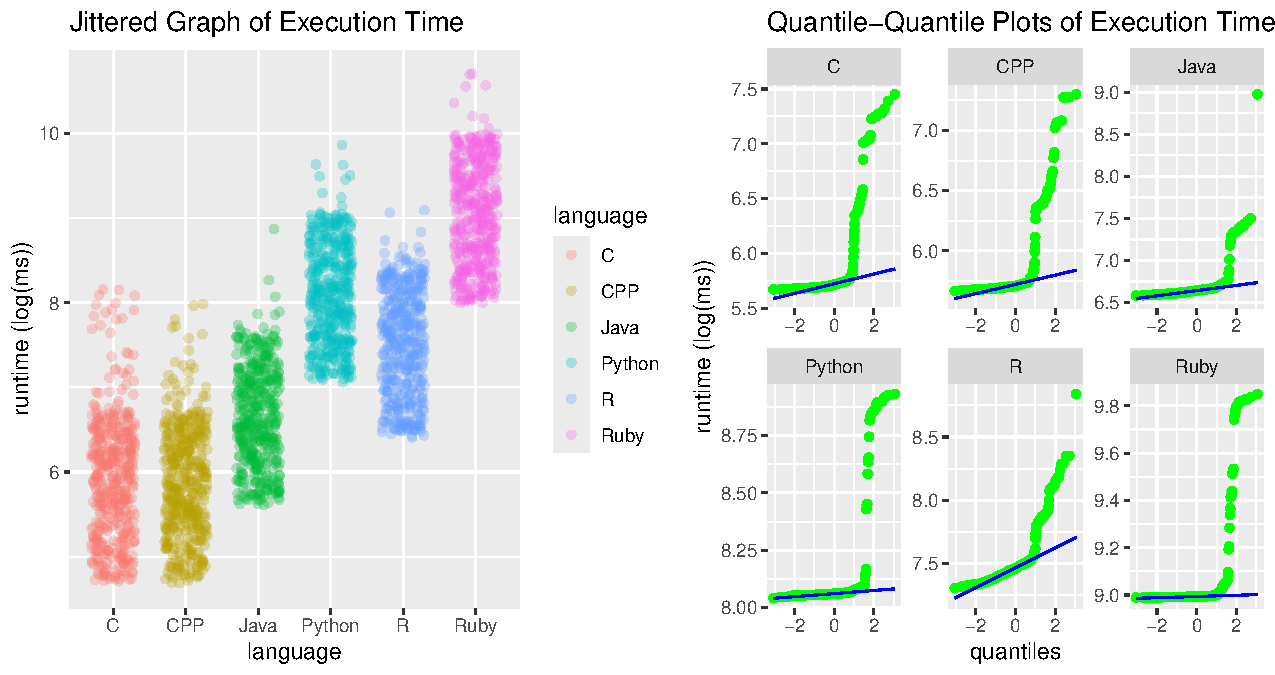
\includegraphics[width=1\linewidth]{skeleton_files/figure-latex/figPrior-1}
We can observe that C and C++ seem to be the fastest languages, though
further analyses are needed. We can also see from the
Quantile-Quantile(QQ) plots that the execution times are clearly not
normally distributed.

\newpage

\section{Methods}\label{methods}

\subsection{Setting}\label{setting}

This study was mostly conducted at the University of Cape Town,
utilising the computers available on campus. We found that there are
only 5 different hardware setups available. Thus, to supplement the
range of our hardware setups, we also borrowed machines of 2 more
hardware setups from our friends.

\subsection{\texorpdfstring{Approximation of
\(\pi\)}{Approximation of \textbackslash pi}}\label{approximation-of-pi}

The number \(\pi\), the ubiquitous and equally mysterious irrational
number, has been fascinating the humankind since time immemorial.
Mathematicians from 4000 years ago to the present time have devised
various methods attempting to get closer to the true value of \(\pi\).
One such method is using Leibniz's formula: \[
4 \left( 1 - \frac{1}{3} + \frac{1}{5} - \frac{1}{7} + \frac{1}{9} ±... \right) = \sum_{k=0}^{\infty}\frac{(-1)^k}{2k+1}
\] Leibniz, whom the formula is named after, proved that the series
above eventually converges to \(\pi\). That is: \[
\pi = 4 \left( 1 - \frac{1}{3} + \frac{1}{5} - \frac{1}{7} + \frac{1}{9} ±... \right) = \sum_{k=0}^{\infty}\frac{(-1)^k}{2k+1}.
\] We applied this algorithm in 6 programming languages, including 3
compiled languages: C, C++, Java, and 3 interpreted languages: Python,
R, Ruby, up to a billion terms.

\subsection{Sources of Variation}\label{sources-of-variation}

\paragraph{Treatments:}\label{treatments}

We have 6 treatment factors, which are the programming languages we
applied algorithm to. Each treatment has one level (applying the formula
up to \(100 \times 10^6\) terms). We selected this particular level
because it is the largest, practical number of terms we could apply with
our hardware setups (For some setups, it may take up to 4 hours to
arrive at a single observation), and fewer terms imply larger relative
measurement error {[}7{]}. We cannot include more levels because in the
existing literature, most studies of such kind choose to run all
languages on the same machine. However, since we would like to avoid
pseudo replication as much as possible we use one machine per
observation. The downside of this approach is that we do not have
sufficient machines to perform more than one levels.

\paragraph{Blocks:}\label{blocks}

From our a priori analysis, we noticed that the execution times of the 6
programming languages we tested seem to follow the same order on various
hardware setups: \begin{equation}
t(C) \approx t(C++) < t(Java) < t(R) < t(Python) < t(Ruby)
\end{equation} Whilst the exact runtimes on machines of the same
hardware setups tend to not vary much. This motivates us to block for
various hardware setups. We also ensured that the machines are all
operating on the same operating system, as we had later found out in the
pilot experiment.

\subsection{Experimental Units:}\label{experimental-units}

As mentioned earlier, we would like to avoid pseudo replication as much
as possible. Therefore, we deviated from the tradition of running all
programming languages on the same machine, and test only one language
per machine. Our experimental units are therefore the individual
machines we ran each test on.

\subsection{Sampling Procedure}\label{sampling-procedure}

Since existing literature tend to suggest that execution times of
programming languages are not normally distributed, we perform a priori
tests to confirm that none of our languages has normally distributed
runtime. This imposed an issue as it prevented us to apply anova models.
To address this, we applied the Central Limit Theorem(CLT) to obtain a
normal distribution for the average execution times. We ran the program
15 times per sample for each programming language, and repeated the
process 30 times. Applying CLT, it is relatively safe to assume the
distribution of sample means is approximately normal {[}2{]}. If we
assume sample means to be normally distributed, the mean of the
distribution of sample means is then an unbiased estimator for the true
run time of each programming language{[}2{]}, which we will take as a
single observation. (Note: We arrived at the number 15 through trial and
error, and 30 from {[}8{]})

\subsection{Randomisation Procedure}\label{randomisation-procedure}

We first order the computers belonging to each block from 1 to 6. We
then used the random number generator from Python's \emph{random} module
to randomly shuffle, and thus producing a permutation of the list, {[}C,
C++, Java, Python, Ruby, R{]}. The index of each programming language in
the permutation would then be paired to the computer with the same
assigned number.

\subsection{Pilot Experiment}\label{pilot-experiment}

We follow this direction and perform an pilot study on 4 differnt
hardware setups to obtain the following data

\begin{verbatim}
## Warning in read.table(file = file, header = header, sep = sep, quote = quote, :
## incomplete final line found by readTableHeader on 'pilotData.csv'
\end{verbatim}

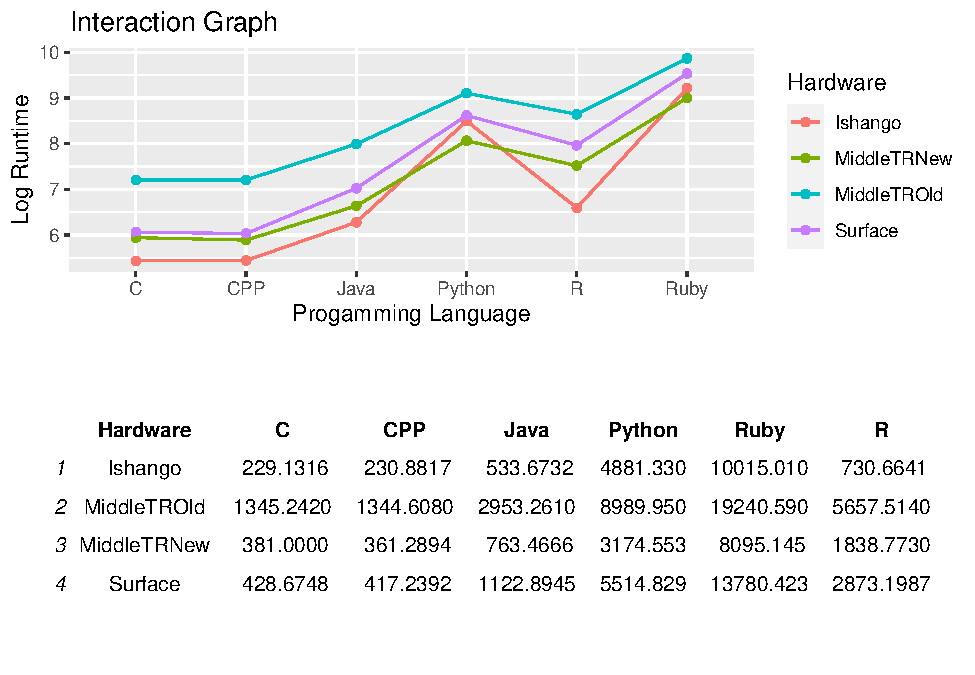
\includegraphics[width=1\linewidth]{skeleton_files/figure-latex/figPilot-1}
From the data collected, we observed that the results collected from
Ishango do not follow the general trends established by the other three
setups. The hardware setup in Ishango lab is significantly less advance
than MiddleTRNew; yet, most programming languages tend to perform better
on the Ishango machine. Secondly, to add to the first observation, not
all programming languages perform better on the Ishango machine.

After further investigation, we learned that programming languages
perform differently on various operating systems {[}4{]}. We
hypothesised that this is likely the reason for the deviation, though
further studies are needed to confirm this (we lack access to machines
with the same hardware setup but run on different operating system).
Therefore, we added another constraint for selecting suitable machines:
the machines must all run on Windows 10, as these machines are the most
widely available.

Besides the observation mentioned above, we can also see that there is
relatively little difference in execution times on the other hardware
setups. This motivates us to employ an Randomised Block Design(RBD)

\subsection{Design}\label{design}

We assume that: \[
e_{ij} \sim \mathcal{N}(0, \sigma^2)
\] We use the following anova model for our response variables:

\[
Y_{ij} = \mu + \alpha_i + \beta_j+ e_{ij}
\] \[
i = 1 ...a
\] \[
j = 1 ...b
\] With the following constraints: \[
\sum_{i=1}^a \alpha_i = \sum_{j=1}^b \beta_i =0 
\] Where: \[
\begin{aligned}
&\mu\hspace{35pt}  \text{overall mean} \\
&\alpha_i\hspace{35pt} \text{effect of }\, i^{th}\, \text{treatment}\\
&\beta_j\hspace{35pt} \text{effect of }\, j^{th}\, \text{block}\\
&e_{ij}\hspace{35pt} \text{random error of the observation}\\
\end{aligned}
\]

We also assume that each \(e_{ij}\) is independent to each other, which
allows us to assume that each \(Y_{ij}\) is also independent to each
other, and are normally distributed. If there are no blocking and
treatment effects, then: \[
Y_{ij} \sim \mathcal{N}(\mu, \sigma^2)
\] Otherwise, if there are blocking and treatment effects, then: \[
Y_{ij} \sim \mathcal{N}(\mu + \alpha_i + \beta_j, \sigma^2)
\]

\newpage

\section{Results}\label{results}

We performed the experiment described above on 7 different hardware
setups and applied all 6 treatments. The table for data and details of
each hardware setups can be found in the appendix. The Analysis of
Variance (ANOVA) table is shown below:

\begin{longtable}[]{@{}lrrrrr@{}}
\toprule\noalign{}
& Df & Sum sq & Mean sq & F value & Pr(\textgreater F) \\
\midrule\noalign{}
\endhead
\bottomrule\noalign{}
\endlastfoot
Language & 5 & 58.1057 & 11.6211 & 1032.9348 & \textless{} 0.0001 \\
Hardware & 6 & 5.5176 & 0.9196 & 81.7379 & \textless{} 0.0001 \\
Residuals & 30 & 0.3375 & 0.0113 & & \\
We verified & our a & ssumptions & by perfor & ming Shapiro & Wilk test
on the residuals. We obtained \\
\end{longtable}

\section{Discussion}\label{discussion}

You can cross-reference sections and subsections as follows: Section
\ref{materials-and-methods} and Section \ref{a-subsection}.

\textbf{\emph{Note:}} the last section in the document will be used as
the section title for the bibliography.

\section{References}\label{references}

\section{Appendix}\label{appendix}

\paragraph{PC Specificiations}\label{pc-specificiations}

\hfill\break

\begin{tabular}{l|r|r|r}
\hline
  & CPU & MEMORY & OPERATING SYSTEM\\
\hline
Ishango PC &  9th Gen Intel® Core™ i3-9100  & 8,0 GB &  Ubuntu 22.04\\
\hline
MidddleTROld & 9th Gen Intel(R) Core(TM) i5-9500 CPU & 8,0 GB &  Windows 10\\
\hline
MiddleTRNew & 12th Gen Intel(R) Core(TM) i5-13400 & 16,0 GB &  Windows 10\\
\hline
ScilabB &  12th Gen Intel(R) Core(TM) i5-12400 &  16,0 GB  &  Windows 10\\
\hline
Surface &  9th Gen Intel(R) Core(TM) i5-8250 CPU &  16,0 GB  &  Windows 10\\
\hline
ASUS laptop &  5th Gen Intel(R) Core(TM) i7-5500U CPU &  6,0 GB  &  Windows 10\\
\end{tabular}

\hfill\break


\begin{notes}[Acknowledgements]
This is an acknowledgement.

It consists of two paragraphs.
\end{notes}




\end{document}
